\documentclass[10pt,a4paper]{article}

\usepackage[utf8]{inputenc}
\usepackage[margin=0.85in]{geometry}
\usepackage{amsmath,amssymb,amsfonts,amsthm}
\usepackage{booktabs}
\usepackage{array}
\usepackage{graphicx}
\usepackage{algorithm}
\usepackage{algpseudocode}
\usepackage[numbers,sort&compress]{natbib}
\usepackage{hyperref}

\pdfinfo{
    /Author ()
    /Title ()
    /Subject ()
    /Keywords ()
}

\hypersetup{
    colorlinks=true,
    linkcolor=blue,
    citecolor=blue,
    urlcolor=black,
    pdfauthor={},
    pdftitle={},
    pdfsubject={},
    pdfkeywords={},
    pdfcreator={},
    pdfproducer={}
}

\newtheorem{theorem}{Theorem}
\newtheorem{lemma}{Lemma}
\newtheorem{proposition}{Proposition}
\newtheorem{corollary}{Corollary}
\newtheorem{remark}{Remark}

\renewcommand{\thesection}{S\arabic{section}}
\renewcommand{\thetable}{S\arabic{table}}
\renewcommand{\thefigure}{S\arabic{figure}}
\renewcommand{\theequation}{S\arabic{equation}}
\renewcommand{\thealgorithm}{S\arabic{algorithm}}

\title{\textbf{Supplementary Material: Optimal age replacement and component-mix design for heterogeneous weighted k-out-of-n:G systems under asymmetric capacity-proportional load sharing}}
\author{}
\date{}

\begin{document}

\maketitle

\noindent This Supplementary Material provides (Section~\ref{sec:S1}) complete formal proofs of Lemma~1, Proposition~1, Remark~1, Theorem~1, Theorem~2, and Remark~2; (Section~\ref{sec:S2}) the two-stage optimization algorithm and the synthetic validation benchmark against the classical independent model \cite{wu1994,nakagawa2005,eryilmaz2014two}; (Section~\ref{sec:S3}) extended mechanism-branch, turning-point, and parameter-box grids for IEEE RTS-GMLC experiments E1--E4; and (Section~\ref{sec:S4}) the full replacement-duration sensitivity grid for E6.

\section*{Abbreviations and Key Notation}
\begin{center}
\footnotesize
\begin{tabular*}{\textwidth}{@{\extracolsep{\fill}}ll|ll@{}}
\toprule
Symbol / Term & Definition & Symbol / Term & Definition \\
\midrule
$\eta(t)$, $\eta_I$, $\eta_{II}$ & Long-run expected cost rate (Policy~I, II) & $\eta_{\mathrm{cal}}(t;\delta,c_d)$ & Calendar cost rate (duty $\delta$, downtime cost $c_d$) \\
$t^*$, $m^*$ & Optimal replacement age and Type~I count & $\Delta\eta\%$ & Naive independence vs.\ load-sharing cost penalty \\
$ind$, $LS$ & Independent baseline vs.\ load sharing & $\mathrm{MTTF}$, $\mathrm{MTTR}$ & Mean time to failure and mean time to repair \\
$\mathrm{FOR}$ & Forced outage rate & $\mathrm{CF}$ & Capacity factor (peaking duty ratio) \\
CTMC, PH & Continuous-Time Markov Chain, Phase-Type & IFR & Increasing Failure Rate \\
PM, CM & Preventive maintenance, corrective maintenance & TFR & Tampered Failure Rate load-sharing law \\
MINLP & Mixed-integer nonlinear program & OEM, $\mathrm{MF}$ & Original equipment manufacturer, maintenance factor \\
CT, HGP & Combustion turbine, hot-gas-path (B/E-class) & RTS-GMLC & IEEE Reliability Test System--GMLC \\
EIA AEO & U.S.\ Energy Info.\ Admin.\ Annual Energy Outlook & O\&M, FOM, VOM & Operation \& maintenance (fixed, variable) \\
\bottomrule
\end{tabular*}
\end{center}

\section{Complete Mathematical Proofs}
\label{sec:S1}

\subsection*{S1.1 Governing Equations Referenced in Proofs}
For self-contained verification, we restate the defining equations from Sections~3.1--3.4 of the main manuscript:
\begin{align}
W_{i,j} &= i w_1 + j w_2, \qquad W_0 = m w_1 + (n - m) w_2, \label{eq:Wij} \\
\lambda_r(i, j) &= \lambda_{r,0} \left( \frac{W_0}{W_{i,j}} \right)^{\gamma_r}, \qquad r \in \{1, 2\}, \label{eq:lam12} \\
R_{sys}^{ind}(t) &= \sum_{i=0}^{m} \sum_{j=0}^{n-m} \mathbb{I}(i w_1 + j w_2 \ge k) \binom{m}{i} \left(e^{-\lambda_{1,0} t}\right)^i \left(1 - e^{-\lambda_{1,0} t}\right)^{m - i} \binom{n - m}{j} \left(e^{-\lambda_{2,0} t}\right)^j \left(1 - e^{-\lambda_{2,0} t}\right)^{n - m - j}, \label{eq:R_ind} \\
R_{sys}(t) &= \boldsymbol{\alpha} \exp(\mathbf{Q}_{\mathcal{W}} t) \mathbf{e} = \sum_{(i,j) \in \mathcal{W}} P_{i,j}(t), \qquad f_{sys}(t) = -\frac{d R_{sys}(t)}{dt} = \boldsymbol{\alpha} \exp(\mathbf{Q}_{\mathcal{W}} t) \mathbf{q}_F, \label{eq:R_sys_f} \\
E[S(t)] &= \int_{0}^{t} R_{sys}(u)\,du = \boldsymbol{\alpha} \mathbf{Q}_{\mathcal{W}}^{-1} \left( \exp(\mathbf{Q}_{\mathcal{W}} t) - \mathbf{I}_M \right) \mathbf{e}, \qquad \mathrm{MTTF} = -\boldsymbol{\alpha} \mathbf{Q}_{\mathcal{W}}^{-1} \mathbf{e}, \label{eq:ES_MTTF} \\
\eta_I(t) &= \frac{c_2 - (c_2 - c_1) R_{sys}(t)}{\int_{0}^{t} R_{sys}(u)\,du}, \qquad 0 < c_1 < c_2. \label{eq:etaI}
\end{align}

\subsection*{S1.2 Lemma 1, Proposition 1, and Remark 1}

\begin{lemma}[Monotonicity of State-Dependent Transition Rates]
For any system state $(i, j) \in \mathcal{W}$ with active capacity $W_{i,j} = i w_1 + j w_2 \ge k$ and sensitivity exponents $\gamma_1, \gamma_2 > 0$:
\begin{enumerate}
    \item $\lambda_1(i, j)$ and $\lambda_2(i, j)$ are strictly decreasing in $i$ and $j$.
    \item For any non-absorbing failure transition $(i, j) \to (i - 1, j) \in \mathcal{W}$ or $(i, j) \to (i, j - 1) \in \mathcal{W}$, the surviving component hazard rates strictly increase:
    $$\lambda_r(i - 1, j) > \lambda_r(i, j) \quad \text{and} \quad \lambda_r(i, j - 1) > \lambda_r(i, j), \quad \forall r \in \{1, 2\}.$$
    \item Whenever both $(i - 1, j) \in \mathcal{W}$ and $(i, j - 1) \in \mathcal{W}$, because $w_2 > w_1$, the hazard jump satisfies $\lambda_r(i, j - 1) > \lambda_r(i - 1, j)$ for all $r \in \{1, 2\}$.
\end{enumerate}
\end{lemma}

\begin{proof}
From (\ref{eq:lam12}), $\lambda_r(i, j) = \lambda_{r,0} (W_0 / W_{i,j})^{\gamma_r}$. Differentiating with respect to $W_{i,j}$ yields:
$$\frac{\partial \lambda_r(i, j)}{\partial W_{i,j}} = -\gamma_r \lambda_{r,0} W_0^{\gamma_r} W_{i,j}^{-(\gamma_r + 1)} < 0 \quad (\text{since } \gamma_r > 0, \, W_{i,j} > 0).$$
Since $\partial W_{i,j} / \partial i = w_1 > 0$ and $\partial W_{i,j} / \partial j = w_2 > 0$, $\partial \lambda_r / \partial i < 0$ and $\partial \lambda_r / \partial j < 0$. Because $W_{i, j-1} = W_{i,j} - w_2 < W_{i,j} - w_1 = W_{i-1, j} < W_{i,j}$ and $(W_0 / W)^{\gamma_r}$ is strictly decreasing in $W$, we obtain $\lambda_r(i, j - 1) > \lambda_r(i - 1, j) > \lambda_r(i, j)$.
\end{proof}

\begin{proposition}[Variance--Drift Decomposition and Unbranched IFR Property]
Let $\mathbf{p}(t) = \frac{\boldsymbol{\alpha} \exp(\mathbf{Q}_{\mathcal{W}} t)}{\boldsymbol{\alpha} \exp(\mathbf{Q}_{\mathcal{W}} t) \mathbf{e}}$ denote the conditional state probability vector given $T_{sys} > t$. Using (\ref{eq:R_sys_f}), the derivative of the system hazard rate $h_{sys}(t) = \mathbf{p}(t)\mathbf{q}_F$ satisfies the exact variance--drift decomposition:
\begin{equation}
\frac{d h_{sys}(t)}{dt} = -\operatorname{Var}_{\mathbf{p}(t)}(\mathbf{q}_F) + \sum_{x \in \mathcal{W}} p_x(t) \sum_{y \neq x, \, y \in \mathcal{W}} Q_{xy} \left(q_{F,y} - q_{F,x}\right),
\label{eq:dh_decomp}
\end{equation}
where $\operatorname{Var}_{\mathbf{p}(t)}(\mathbf{q}_F) = \sum_{x \in \mathcal{W}} p_x(t) q_{F,x}^2 - [h_{sys}(t)]^2 \ge 0$. Eq.~(\ref{eq:dh_decomp}) gives the exact pointwise competition governing whether $dh_{sys}(t)/dt$ is positive at time $t$. Unconditionally, whenever the initial capacity margin satisfies $W_0 - k \ge \min\{w_r : \text{type } r \text{ present}\}$ ($M \ge 2$), $T_{sys}$ is strictly Increasing Failure Rate (IFR) whenever the operational chain reduces to an unbranched series of $M_{\mathrm{eff}} \ge 2$ phases: either $m=0$ or $m=n$ (with $M_{\mathrm{eff}} = M$), or the homogeneous symmetric limit $w_1=w_2, \lambda_{1,0}=\lambda_{2,0}, \gamma_1=\gamma_2$ (lumped over $i+j$ into $M_{\mathrm{eff}} = n - \lceil k/w_1 \rceil + 1$ phases).
\end{proposition}

\begin{proof}
Differentiating $\mathbf{p}(t) = \mathbf{P}_{\mathcal{W}}(t)/R_{sys}(t)$ using $\mathbf{P}_{\mathcal{W}}'(t) = \mathbf{P}_{\mathcal{W}}(t)\mathbf{Q}_{\mathcal{W}}$ and $R_{sys}'(t) = -h_{sys}(t)R_{sys}(t)$ gives:
$$\frac{d\mathbf{p}(t)}{dt} = \mathbf{p}(t)\mathbf{Q}_{\mathcal{W}} + h_{sys}(t)\mathbf{p}(t), \quad \frac{d h_{sys}(t)}{dt} = \mathbf{p}(t)\mathbf{Q}_{\mathcal{W}}\mathbf{q}_F + [h_{sys}(t)]^2.$$
Because row sums of the full CTMC generator equal zero, $Q_{xx} = -\left(\sum_{y \neq x, y \in \mathcal{W}} Q_{xy} + q_{F,x}\right)$ for each $x \in \mathcal{W}$. Substituting $Q_{xx}$ into $(\mathbf{Q}_{\mathcal{W}}\mathbf{q}_F)_x$ yields:
$$(\mathbf{Q}_{\mathcal{W}}\mathbf{q}_F)_x = -\left(\sum_{y \neq x} Q_{xy} + q_{F,x}\right)q_{F,x} + \sum_{y \neq x} Q_{xy} q_{F,y} = -q_{F,x}^2 + \sum_{y \neq x} Q_{xy}(q_{F,y} - q_{F,x}).$$
Multiplying by $p_x(t)$, summing over $x \in \mathcal{W}$, and adding $[h_{sys}(t)]^2$ produces (\ref{eq:dh_decomp}):
$$\frac{dh_{sys}(t)}{dt} = -\left(\sum_{x \in \mathcal{W}} p_x(t) q_{F,x}^2 - [h_{sys}(t)]^2\right) + \sum_{x \in \mathcal{W}} p_x(t)\sum_{y \neq x} Q_{xy}(q_{F,y} - q_{F,x}).$$
In the unbranched case with $M_{\mathrm{eff}} \ge 2$ (where $M_{\mathrm{eff}} = M$ for single-type arrays $m \in \{0, n\}$ and $M_{\mathrm{eff}} = n - \lceil k/w_1 \rceil + 1 \le M$ for the lumped homogeneous symmetric chain over $i + j$), $T_{sys}$ is a finite convolution of $M_{\mathrm{eff}}$ independent exponential sojourn times, which is unconditionally log-concave and therefore strictly IFR ($dh_{sys}(t)/dt > 0$ for all $t > 0$).
\end{proof}

\begin{remark}[Non-monotonic Hazard Rates in Branching Two-Type Chains]
Eq.~(\ref{eq:dh_decomp}) reveals why general branching acyclic PH distributions are \emph{not} universally IFR: the survivor-selection variance $-\operatorname{Var}_{\mathbf{p}(t)}(\mathbf{q}_F) \le 0$ pulls $h_{sys}(t)$ downward whenever parallel paths exhibit unequal absorption rates. In heterogeneous two-type systems, Type~I dominated boundary states (e.g., $(5,5)$ at $k=15$) possess higher absorption rates than Type~II dominated boundary states (e.g., $(0,8)$). As fast-absorbing Type~I paths fail, late-time survival conditions onto slower Type~II paths and allows $dh_{sys}(t)/dt < 0$ over localized tail intervals for $m \in \{5, 6, 8\}$ in Figure~\ref{fig:S1}c ($t \in [17.6, 22.4]$ at $m=5$, where $R_{sys}(17.6) = 3.32 \times 10^{-6}$; $[14.6, 33.0]$ at $m=6$, $R_{sys}(14.6) = 2.12 \times 10^{-5}$; and $[9.7, 14.2]$ at $m=8$, $R_{sys}(9.7) = 2.80 \times 10^{-4}$), and across the asymptotic tail $t \ge 14.0$ for $m = 7$ (monotonically approaching the slowest boundary exit rate $\nu_{(0,8)} = 0.9592$ from above and truncated at $t = 36.7$ by the $R_{sys}(t) = 10^{-15}$ survival-precision floor, where $R_{sys}(14.0) = 1.04 \times 10^{-5}$). Because these tail decreases occur at negligible survival probabilities beyond the optimal preventive age ($t^* \in [1.42, 2.10]$ across $m \in \{5, 6, 7, 8\}$), Algorithm~\ref{alg:opt} locates global minima reliably via its dense global grid. If $W_0 - k < \min\{w_r : \text{type } r \text{ present}\}$ (e.g., $m=15, W_0=k=15$), then $M=1$ and $T_{sys}$ is exponential with $dh_{sys}(t)/dt \equiv 0$.
\end{remark}

\subsection*{S1.3 Theorem 1, Theorem 2, and Remark 2}

\begin{theorem}[Existence and Uniqueness Conditions for Policy~I Optimal Age $t^*$]
Under Policy~I with replacement costs $0 < c_1 < c_2$ and $M \ge 2$, every interior stationary point $t^* \in (0, \infty)$ of $\eta_I(t)$ in (\ref{eq:etaI}) satisfies the necessary condition:
\begin{equation}
g(t^*) = h_{sys}(t^*) \int_{0}^{t^*} R_{sys}(u)\,du - [1 - R_{sys}(t^*)] - \frac{c_1}{c_2 - c_1} = 0.
\label{eq:opt_condition}
\end{equation}
If $\lim_{t \to \infty} h_{sys}(t) \cdot \mathrm{MTTF} > \frac{c_2}{c_2 - c_1}$, at least one finite root $t^* \in (0, \infty)$ exists. Under the unbranched IFR condition of Proposition~1 ($h_{sys}'(t) > 0$ for all $t > 0$):
\begin{enumerate}
    \item $t^*$ is the unique finite root of (\ref{eq:opt_condition}) and the strict global minimum ($\eta_I''(t^*) > 0$) whenever $\lim_{t \to \infty} h_{sys}(t) \cdot \mathrm{MTTF} > \frac{c_2}{c_2 - c_1}$.
    \item If $\lim_{t \to \infty} h_{sys}(t) \cdot \mathrm{MTTF} \le \frac{c_2}{c_2 - c_1}$, then $g(t) < 0$ for all $t > 0$, $\eta_I(t)$ is strictly decreasing, and corrective-only replacement ($t^* \to \infty$) is optimal.
\end{enumerate}
\end{theorem}

\begin{proof}
Differentiating $\eta_I(t)$ in (\ref{eq:etaI}) with respect to $t$ and using $R_{sys}'(t) = -h_{sys}(t) R_{sys}(t)$ gives:
$$\frac{d \eta_I(t)}{dt} = \frac{R_{sys}(t)(c_2 - c_1)}{\left(\int_{0}^{t} R_{sys}(u)\,du\right)^2} \, g(t).$$
Hence stationary points satisfy $g(t) = 0$ (\ref{eq:opt_condition}). Evaluating limits using (\ref{eq:ES_MTTF}) yields $\lim_{t \to 0^+} g(t) = -\frac{c_1}{c_2 - c_1} < 0$ and $\lim_{t \to \infty} g(t) = \left(\lim_{t \to \infty} h_{sys}(t)\right) \mathrm{MTTF} - \frac{c_2}{c_2 - c_1}$. By the Intermediate Value Theorem, $\lim_{t \to \infty} h_{sys}(t) \cdot \mathrm{MTTF} > \frac{c_2}{c_2 - c_1}$ guarantees at least one finite root $t^* \in (0, \infty)$. Differentiating $g(t)$ yields:
$$g'(t) = h_{sys}'(t) \int_{0}^{t} R_{sys}(u)\,du + h_{sys}(t) R_{sys}(t) - f_{sys}(t) = h_{sys}'(t) \int_{0}^{t} R_{sys}(u)\,du.$$
Under the IFR condition $h_{sys}'(t) > 0$, $g'(t) > 0$ for all $t > 0$, making $g(t)$ strictly increasing on $(0, \infty)$; thus $t^*$ is unique and $\eta_I''(t^*) > 0$ if the boundary condition holds, whereas $g(t) < 0$ everywhere otherwise. For general branching systems where $h_{sys}'(t)$ may become negative in the tail, uniqueness is not guaranteed analytically and global optimality is resolved numerically via Algorithm~\ref{alg:opt}.
\end{proof}

\begin{theorem}[Boundary Limits Under Load-Sharing Extremes]
Let $t^*(\gamma_1, \gamma_2)$ denote the optimal replacement age under Policy~I with exponents $(\gamma_1, \gamma_2)$ over compact bracket $[t_{lb}, t_{ub}]$ (or corrective-only fallback $\infty$). Then:
\begin{enumerate}
    \item \textbf{Independent Limit:} As $\gamma_1, \gamma_2 \to 0$, $R_{sys}(t) \to R_{sys}^{ind}(t)$ and $\eta_I(t) \to \eta_I^{ind}(t)$ uniformly on $[t_{lb}, t_{ub}]$. Whenever the baseline minimizer $t_{ind}^* \in (t_{lb}, t_{ub})$ is unique (or corrective-only replacement is strictly preferred), $t^*(\gamma_1, \gamma_2) \to t_{ind}^*$.
    \item \textbf{Weakest-Link Limit:} As $\gamma_1, \gamma_2 \to \infty$, any component failure drives surviving units in degraded states $(i, j) \neq (m, n-m)$ to unbounded hazard rates ($\lambda_r \to \infty$), collapsing the lifetime distribution to the memoryless first-failure law:
    $$\lim_{\gamma_1, \gamma_2 \to \infty} R_{sys}(t) = \exp\left( -(m \lambda_{1,0} + (n - m) \lambda_{2,0}) t \right).$$
    In this limit, $h_{sys}(t) = m \lambda_{1,0} + (n - m) \lambda_{2,0}$ is constant, $g(t) < 0$ for all $t > 0$, and $t^*(\gamma_1, \gamma_2) \to \infty$ (corrective-only replacement).
\end{enumerate}
\end{theorem}

\begin{proof}
For part~1, letting $(\gamma_1, \gamma_2) \to (0, 0)$ in (\ref{eq:lam12}) sends $\mathbf{Q}_{\mathcal{W}}(\gamma_1, \gamma_2) \to \mathbf{Q}_{\mathcal{W}}(0, 0)$ continuously; by continuity of the matrix exponential and matrix inverse, $R_{sys}(t) \to R_{sys}^{ind}(t)$ and $\int_0^t R_{sys}(u)\,du$ converge uniformly on any compact interval $[t_{lb}, t_{ub}] \subset (0, \infty)$. Uniform convergence of continuous $\eta_I(\cdot; \gamma_1, \gamma_2)$ to $\eta_I^{ind}(\cdot)$ on compact $[t_{lb}, t_{ub}]$ ensures $\arg\min_{t \in [t_{lb}, t_{ub}]} \eta_I(t; \gamma_1, \gamma_2) \to t_{ind}^*$ whenever $t_{ind}^*$ is the unique minimizer (and similarly $\eta_I^{ind} > \eta(\infty)$ preserves corrective-only convergence). For part~2, partition $\mathcal{W} = \{x_0\} \cup \mathcal{W}_{\mathrm{deg}}$ into the intact initial state $x_0 = (m, n - m)$ (with constant exit rate $\nu_0 = m\lambda_{1,0} + (n - m)\lambda_{2,0}$) and the non-empty degraded subset $\mathcal{W}_{\mathrm{deg}}$ (for $M \ge 2$). Conformably partitioning $\mathbf{Q}_{\mathcal{W}} = \begin{pmatrix} -\nu_0 & \mathbf{q}_{0,\mathrm{deg}} \\ \mathbf{0} & \mathbf{Q}_{\mathrm{deg}} \end{pmatrix}$ and setting $\underline{\lambda} = \min(\lambda_{1,0}, \lambda_{2,0}) > 0$ and $\rho_{\min} = \min_{(i,j)\in\mathcal{W}_{\mathrm{deg}}} W_0/W_{i,j} > 1$, every degraded total exit rate satisfies $\nu_{i,j} \ge \underline{\lambda}\,\rho_{\min}^{\min(\gamma_1,\gamma_2)} \to \infty$ as $\gamma_1, \gamma_2 \to \infty$. Writing $\mathbf{Q}_{\mathrm{deg}} = -\mathbf{D}_{\mathrm{deg}}(\mathbf{I} - \mathbf{N})$ with diagonal $\mathbf{D}_{\mathrm{deg}} = \operatorname{diag}(\nu_{i,j})$ and strictly upper-triangular substochastic matrix $\mathbf{N}$ satisfying $\mathbf{N}^{M-1} = \mathbf{0}$ and $\|\mathbf{N}\|_\infty \le 1$, the Neumann expansion gives $\|\mathbf{Q}_{\mathrm{deg}}^{-1}\|_\infty \le (M - 1)/\min_{(i,j)\in\mathcal{W}_{\mathrm{deg}}} \nu_{i,j} \to 0$. Similarly, by Duhamel's formula on the block generator, the transition submatrix satisfies $\|\exp(\mathbf{Q}_{\mathrm{deg}} t)\|_\infty \to 0$ uniformly on $[\epsilon, \infty)$ for every $\epsilon > 0$. Consequently, $R_{sys}(t; \gamma_1, \gamma_2) \to e^{-\nu_0 t}$ and $f_{sys}(t; \gamma_1, \gamma_2) \to \nu_0 e^{-\nu_0 t}$ uniformly on every compact interval $[t_{lb}, t_{ub}] \subset (0, \infty)$, while $\mathrm{MTTF}(\gamma_1, \gamma_2) = \nu_0^{-1} - \mathbf{q}_{0,\mathrm{deg}}\nu_0^{-1}\mathbf{Q}_{\mathrm{deg}}^{-1}\mathbf{e} \to \nu_0^{-1}$. Since the limit cost rate $\eta_{I,\infty}(t) = \nu_0(c_2 - c_1) + \frac{\nu_0 c_1}{1 - e^{-\nu_0 t}}$ is strictly decreasing on $(0, \infty)$ with $\eta_{I,\infty}'(t) = -\frac{\nu_0^2 c_1 e^{-\nu_0 t}}{(1 - e^{-\nu_0 t})^2} < 0$ and $\lim_{t\to\infty}\eta_{I,\infty}(t) = \nu_0 c_2$, uniform convergence ensures $\eta_I'(t; \gamma_1, \gamma_2) \to \eta_{I,\infty}'(t) < 0$ uniformly on $[t_{lb}, t_{ub}]$ and $\inf_{t \in [t_{lb}, t_{ub}]} \eta_I(t; \gamma_1, \gamma_2) > \eta_I(\infty; \gamma_1, \gamma_2)$ for all sufficiently large $\gamma_1, \gamma_2$, forcing $t^*(\gamma_1, \gamma_2) = \infty$ without invoking Theorem~1 on the limit chain.
\end{proof}

\begin{remark}[Empirical Turning Point Between Boundary Limits]
Theorem~2 establishes only the two extreme limits ($\gamma \to 0$ and $\gamma \to \infty$) rather than proving unimodality across intermediate exponents. Numerically, however, moderate $\gamma$ accelerates multi-stage degradation and lowers $t^*$ below $t_{ind}^*$, whereas larger $\gamma$ progressively concentrates survival risk on the first failure toward the memoryless weakest-link limit where $h_\infty \cdot \mathrm{MTTF} \le \frac{c_2}{c_2-c_1}$. Between these limits, $t^*(\gamma)$ passes an empirical turning point and rises toward $\infty$, observed near $\gamma \approx 18$ and $\gamma \approx 30.08$ in Section~\ref{sec:S2} and across IEEE RTS-GMLC arrays in Section~5.2 of the main text.
\end{remark}

\section{Optimization Algorithm and Synthetic Validation Benchmark}
\label{sec:S2}

Algorithm~\ref{alg:opt} details the two-stage grid-bracketed global-to-local solver designed to prevent tail traps when bounded Brent probes land on the flat asymptote $R_{sys}(t) \approx 0$.

\begin{algorithm}[htbp]
\caption{Two-stage grid-bracketed component-mix and age replacement optimization.}
\label{alg:opt}
\begin{algorithmic}[1]
\Require Total units $n$; weights $w_1, w_2$; threshold $k$; baseline rates $\lambda_{1,0}, \lambda_{2,0}$; exponents $\gamma_1, \gamma_2$; cost parameters and durations $(d_{PM}, d_{CM})$; search bounds $(t_{lb}, t_{ub})$; grid size $N_{grid} = 300$.
\Ensure Optimal mix $m^*$, optimal replacement age $t^*$, minimum cost rate $\eta^*$.
\State Initialize $\eta_{\min} \gets \infty$, $m^* \gets -1$, $t^* \gets -1$.
\For{$m = 0$ \textbf{to} $n$}
    \State Compute nominal capacity $W_0 \gets m w_1 + (n - m) w_2$;
    \If{$W_0 < k$} \textbf{continue}; \EndIf
    \State Construct operational state space $\mathcal{W}$ and generator $\mathbf{Q}_{\mathcal{W}}$ via (\ref{eq:lam12});
    \State Compute $\mathrm{MTTF}$ and corrective-only asymptote $\eta(\infty)$;
    \If{$M = 1$ \textbf{and} $d_{PM} = d_{CM} = 0$ \textbf{and} $\eta(m, \max(t_{lb}, 0.5\,\mathrm{MTTF})) > \eta(\infty)$}
        \State $t_m \gets \infty$, $\eta_{\mathrm{val}} \gets \eta(\infty)$; \Comment{Exponential single-state system: corrective-only}
    \Else
        \State Build two-segment uniform grid of $N_{grid}$ points: $\lfloor 0.75 N_{grid} \rfloor$ points on $[t_{lb}, t_{\mathrm{split}})$ and $N_{grid} - \lfloor 0.75 N_{grid} \rfloor$ points on $[t_{\mathrm{split}}, t_{\max}]$, where $t_{\max} = \max(t_{ub}, 6\,\mathrm{MTTF})$ and $t_{\mathrm{split}} = \min(t_{\max}, 3\,\mathrm{MTTF})$;
        \State Evaluate $\eta(m, t_g)$ for $g = 1, \dots, N_{grid}$, set $N_{\mathrm{last}} \gets N_{grid}$ and $g^* \gets \arg\min_{g} \eta(m, t_g)$;
        \If{$g^* = N_{grid}$ \textbf{and} $\eta(m, t_{g^*}) < \eta(\infty) - 10^{-12}$}
            \State Append $N_{\mathrm{ext}} - 1$ uniform points over $(t_{\max}, \max(3\,t_{\max}, 20\,\mathrm{MTTF})]$ (with $N_{\mathrm{ext}} = \max(60, \lfloor N_{grid}/2 \rfloor)$), update $N_{\mathrm{last}} \gets N_{grid} + N_{\mathrm{ext}} - 1$ and $g^*$;
        \EndIf
        \If{$g^* = N_{\mathrm{last}}$ \textbf{or} $\eta(m, t_{g^*}) \ge \eta(\infty) - 10^{-12}$}
            \State $t_m \gets \infty$, $\eta_{\mathrm{val}} \gets \eta(\infty)$;
        \Else
            \State Refine $t_m \gets \arg\min_{t \in [t_{\max(1, g^*-1)}, t_{g^*+1}]} \eta(m, t)$ via bounded Brent search (absolute tolerance $10^{-9}$);
            \State Set $\eta_{\mathrm{val}} \gets \eta(m, t_m)$ (retaining grid minimum $t_{g^*}$ if strictly lower) and return $\infty$ if $\eta_{\mathrm{val}} \ge \eta(\infty) - 10^{-12}$;
        \EndIf
    \EndIf
    \If{$\eta_{\mathrm{val}} < \eta_{\min}$}
        \State $\eta_{\min} \gets \eta_{\mathrm{val}}$, $m^* \gets m$, $t^* \gets t_m$;
    \EndIf
\EndFor
\State \Return $m^*, t^*, \eta_{\min}$
\end{algorithmic}
\end{algorithm}

To verify exact concordance with the classical independent weighted $k$-out-of-$n$:G age-replacement formulation \cite{wu1994,nakagawa2005,eryilmaz2014two}, Tables~\ref{tab:S1}--\ref{tab:S4} and Figures~\ref{fig:S1}--\ref{fig:S4} evaluate the dimensionless synthetic parameter set $w_1 = 1$, $w_2 = 2$, $\lambda_{1,0} = 0.2$, $\lambda_{2,0} = 0.1$ (matching the two-type baseline in Eryilmaz and Sarikaya \cite{eryilmaz2014two}), $c_1 = 1.0$, $c_2 = 5.0$ (Policy~I, $(t_{lb}, t_{ub}) = (0.01, 20)$), and $c_0 = 0.5$, $c_{pen} = 3.0$, $c_{rep,1} = 0.15$, $c_{rep,2} = 1.05$, $c_{ref,1} = 0.02$, $c_{ref,2} = 0.08$ (Policy~II, $(t_{lb}, t_{ub}) = (0.05, 15)$). Under $\gamma_1 = \gamma_2 = 0$, Table~\ref{tab:S1} matches the analytical double-binomial formulation (\ref{eq:R_ind}) to machine precision across all 16 configurations (covering $k \in \{8, 10, 13, 17, 20\}$ on $n=15, m=5$, with maximum relative error $\max_{t \in [0.1, 10.0]} |R_{sys}(t) - R_{sys}^{ind}(t)| / R_{sys}^{ind}(t) \le 5.302 \times 10^{-15}$ over 50 points). Under load sharing ($n = 15, k = 15$, Table~\ref{tab:S2} and Figures~\ref{fig:S1}--\ref{fig:S2}), neglecting load redistribution produces overly long replacement ages and economic penalties up to 19.58\% at $m = 3$ under Regime~3 ($\gamma_1 = \gamma_2 = 1.5$). Under Policy~II (Table~\ref{tab:S3} and Figure~\ref{fig:S3}), unit cost differentiation yields global optimum $m^* = 4$ ($\eta_{II}^* = 1.8082$, $t^* = 3.038$; near-tie $m = 3$ at $1.8083$). Finally, Table~\ref{tab:S4} and Figure~\ref{fig:S4} confirm steeper sensitivity to $\gamma_2$ than $\gamma_1$ when $w_2 = 2 w_1$; extending $\gamma_1 = \gamma_2$ past Table~\ref{tab:S4} places the turning point near $\gamma \approx 18$ ($t^* \approx 0.425$) and the bifurcation to $t^* = \infty$ near $\gamma \approx 30.08$, where $h_\infty \cdot \mathrm{MTTF} \le \frac{c_2}{c_2-c_1} = 1.25$. To cross-check the PH matrix-exponential implementation at $\gamma > 0$, independent $100{,}000$-trajectory Monte Carlo CTMC jump simulations (\texttt{mc\_validation\_gamma\_gt0.csv}, 8 cases, fixed seed \texttt{42}) match analytical PH $\mathrm{MTTF}$ within $0.026\%$--$0.514\%$ and survival probability error $|R_{sys}^{\mathrm{MC}}(t) - R_{sys}(t)|$ within $0.0001$--$0.0026$ across Synthetic Regimes~1--3, CT Area~1 at $k/W_0 = 0.70$ ($\gamma \in \{4.96, 12.88\}$, including asymmetric pairs), and deep-cascade CT Area~1 at $k/W_0 = 0.50$ ($\gamma \in \{23.45, 60.90\}$), while Pad\'e scaling-and-squaring matrix exponentials with overflow-guarded log-hazard cap $\gamma_r \ln(W_0/W_{i,j}) \le 650$ preserve numerical conditioning at high $\gamma$.

\begin{table}[htbp]
\centering
\footnotesize
\caption{Baseline benchmark validation under the classical independent model ($\gamma_1 = \gamma_2 = 0$, matching \texttt{synthetic\_table2\_baseline.csv}).}
\label{tab:S1}
\begin{tabular*}{\textwidth}{@{\extracolsep{\fill}}lccccccccc@{}}
\toprule
Scenario & Total $n$ & Threshold $k$ & Type I $m$ & Type II $n-m$ & Capacity $W_0$ & Margin $W_0-k$ & $t^*$ & $\eta^*$ & Max Rel.\ Err. \\
\midrule
S1  & 10 & 10 &  8 &  2 & 12 &  2 & 0.968 & 2.363 & 1.409e-15 \\
S2  & 10 & 12 &  6 &  4 & 14 &  2 & 1.098 & 2.468 & 1.621e-15 \\
S3  & 10 & 15 &  3 &  7 & 17 &  2 & 1.206 & 2.519 & 2.171e-15 \\
S4  & 15 & 15 &  3 & 12 & 27 & 12 & 3.106 & 0.427 & 1.100e-15 \\
S5  & 15 & 15 &  5 & 10 & 25 & 10 & 2.521 & 0.540 & 1.221e-15 \\
S6  & 15 & 15 &  7 &  8 & 23 &  8 & 1.962 & 0.720 & 1.375e-15 \\
S7  & 15 & 15 & 12 &  3 & 18 &  3 & 0.768 & 2.359 & 2.182e-15 \\
S8  & 15 & 15 & 13 &  2 & 17 &  2 & 0.589 & 3.611 & 5.302e-15 \\
S9  & 15 & 10 & 15 &  0 & 15 &  5 & 1.234 & 1.117 & 2.269e-15 \\
S10 & 15 & 15 & 14 &  1 & 16 &  1 & 0.490 & 6.541 & 3.481e-15 \\
S11 & 15 & 20 &  7 &  8 & 23 &  3 & 0.835 & 2.574 & 1.641e-15 \\
S12 & 15 &  8 &  5 & 10 & 25 & 17 & 5.858 & 0.213 & 1.433e-15 \\
S13 & 15 & 10 &  5 & 10 & 25 & 15 & 4.637 & 0.273 & 1.333e-15 \\
S14 & 15 & 13 &  5 & 10 & 25 & 12 & 3.251 & 0.404 & 8.645e-16 \\
S15 & 15 & 17 &  5 & 10 & 25 &  8 & 1.908 & 0.755 & 1.372e-15 \\
S16 & 15 & 20 &  5 & 10 & 25 &  5 & 1.185 & 1.439 & 2.167e-15 \\
\bottomrule
\end{tabular*}
\end{table}

\begin{table}[htbp]
\centering
\footnotesize
\caption{Synthetic Policy~I load-sharing comparison and naive-schedule penalty $\Delta\eta\%$ ($n = 15, k = 15$).}
\label{tab:S2}
\begin{tabular*}{\textwidth}{@{\extracolsep{\fill}}lccccccr@{}}
\toprule
Mix ($m$) & Regime & $\gamma_1$ & $\gamma_2$ & $t_{LS}^*$ & $\eta_{LS}^*$ & Naive $\eta(t_{ind}^*)$ & Penalty ($\Delta\eta\%$) \\
\midrule
3  & Regime 0 & 0.0 & 0.0 & 3.106 & 0.427 & 0.427 & 0.00\% \\
3  & Regime 1 & 0.8 & 0.8 & 2.500 & 0.528 & 0.560 & 6.05\% \\
3  & Regime 2 & 1.5 & 0.5 & 2.593 & 0.509 & 0.530 & 4.16\% \\
3  & Regime 3 & 1.5 & 1.5 & 2.091 & 0.631 & 0.754 & 19.58\% \\
\midrule
5  & Regime 0 & 0.0 & 0.0 & 2.521 & 0.540 & 0.540 & 0.00\% \\
5  & Regime 1 & 0.8 & 0.8 & 2.084 & 0.651 & 0.677 & 4.05\% \\
5  & Regime 2 & 1.5 & 0.5 & 2.096 & 0.648 & 0.673 & 3.75\% \\
5  & Regime 3 & 1.5 & 1.5 & 1.781 & 0.762 & 0.862 & 13.21\% \\
\midrule
7  & Regime 0 & 0.0 & 0.0 & 1.962 & 0.720 & 0.720 & 0.00\% \\
7  & Regime 1 & 0.8 & 0.8 & 1.671 & 0.843 & 0.864 & 2.49\% \\
7  & Regime 2 & 1.5 & 0.5 & 1.631 & 0.863 & 0.891 & 3.27\% \\
7  & Regime 3 & 1.5 & 1.5 & 1.462 & 0.963 & 1.042 & 8.18\% \\
\midrule
12 & Regime 0 & 0.0 & 0.0 & 0.768 & 2.359 & 2.359 & 0.00\% \\
12 & Regime 1 & 0.8 & 0.8 & 0.715 & 2.527 & 2.533 & 0.25\% \\
12 & Regime 2 & 1.5 & 0.5 & 0.682 & 2.636 & 2.653 & 0.67\% \\
12 & Regime 3 & 1.5 & 1.5 & 0.672 & 2.681 & 2.703 & 0.82\% \\
\bottomrule
\end{tabular*}
\end{table}

\begin{table}[htbp]
\centering
\footnotesize
\caption{Synthetic Policy~II component-mix optimization ($n = 15, k = 15, \gamma_1 = 1.5, \gamma_2 = 0.5$).}
\label{tab:S3}
\begin{tabular*}{\textwidth}{@{\extracolsep{\fill}}cccccccc@{}}
\toprule
Mix ($m$) & Type I $m$ & Type II $n-m$ & Capacity $W_0$ & Margin $W_0-k$ & $\mathrm{MTTF}$ & $t_{II}^*$ & $\eta_{II}^*$ \\
\midrule
0  &  0 & 15 & 30 & 15 & 6.19 & 4.538 & 1.8642 \\
1  &  1 & 14 & 29 & 14 & 5.82 & 4.141 & 1.8389 \\
2  &  2 & 13 & 28 & 13 & 5.43 & 3.769 & 1.8192 \\
3  &  3 & 12 & 27 & 12 & 5.03 & 3.405 & 1.8083 \\
\textbf{4} & \textbf{4} & \textbf{11} & \textbf{26} & \textbf{11} & \textbf{4.60} & \textbf{3.038} & \textbf{1.8082 (Optimum)} \\
5  &  5 & 10 & 25 & 10 & 4.17 & 2.673 & 1.8190 \\
6  &  6 &  9 & 24 &  9 & 3.72 & 2.328 & 1.8420 \\
7  &  7 &  8 & 23 &  8 & 3.29 & 2.011 & 1.8814 \\
8  &  8 &  7 & 22 &  7 & 2.86 & 1.720 & 1.9450 \\
9  &  9 &  6 & 21 &  6 & 2.46 & 1.454 & 2.0452 \\
10 & 10 &  5 & 20 &  5 & 2.07 & 1.210 & 2.2042 \\
11 & 11 &  4 & 19 &  4 & 1.70 & 0.987 & 2.4646 \\
12 & 12 &  3 & 18 &  3 & 1.35 & 0.786 & 2.9187 \\
13 & 13 &  2 & 17 &  2 & 1.01 & 0.614 & 3.8024 \\
14 & 14 &  1 & 16 &  1 & 0.67 & 0.531 & 5.8749 \\
15 & 15 &  0 & 15 &  0 & 0.33 & $\infty$ (CM) & 11.7900 \\
\bottomrule
\end{tabular*}
\end{table}

\begin{table}[htbp]
\centering
\footnotesize
\caption{Synthetic sensitivity analysis over load-sharing exponents ($n = 15, k = 15, m = 5$).}
\label{tab:S4}
\begin{tabular*}{\textwidth}{@{\extracolsep{\fill}}ccccc@{}}
\toprule
$\gamma_1$ & $\gamma_2$ & $\mathrm{MTTF}$ & Optimal replacement age $t^*$ & Minimum cost rate $\eta^*$ \\
\midrule
0.0 & 0.0 & 5.01 & 2.521 & 0.540 \\
0.5 & 0.5 & 4.42 & 2.235 & 0.608 \\
1.0 & 1.0 & 3.92 & 1.991 & 0.681 \\
1.5 & 0.5 & 4.17 & 2.096 & 0.648 \\
0.5 & 1.5 & 3.69 & 1.879 & 0.721 \\
1.5 & 1.5 & 3.51 & 1.781 & 0.762 \\
2.0 & 2.0 & 3.15 & 1.599 & 0.849 \\
3.0 & 3.0 & 2.60 & 1.307 & 1.045 \\
3.5 & 3.5 & 2.38 & 1.190 & 1.155 \\
\bottomrule
\end{tabular*}
\end{table}

\begin{figure}[htbp]
\centering
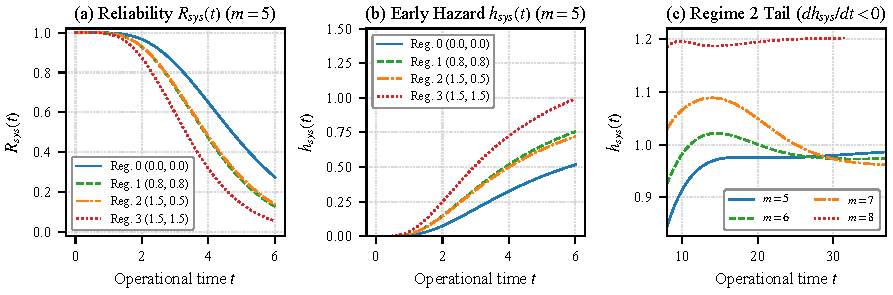
\includegraphics[width=0.98\textwidth]{../figures/figS1_reliability_hazard.pdf}
\caption{Synthetic benchmark ($n = 15, k = 15$): (a) system reliability function $R_{sys}(t)$ at $m = 5$; (b) early system hazard rate $h_{sys}(t)$ at $m = 5$ under Regimes~0--3; and (c) late-time Regime~2 hazard rate $h_{sys}(t)$ ($t \in [8, 37]$) for $m \in \{5, 6, 7, 8\}$ illustrating localized non-monotonic tail intervals where $dh_{sys}(t)/dt < 0$.}
\label{fig:S1}
\end{figure}

\begin{figure}[htbp]
\centering
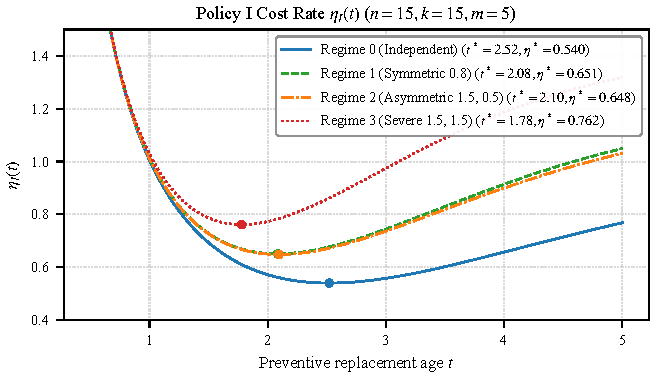
\includegraphics[width=0.72\textwidth]{../figures/figS2_cost_convexity.pdf}
\caption{Synthetic benchmark ($n = 15, k = 15, m = 5$): Policy~I long-run expected cost rate $\eta_I(t)$ with circular markers at global minimizers $t^*$.}
\label{fig:S2}
\end{figure}

\begin{figure}[htbp]
\centering
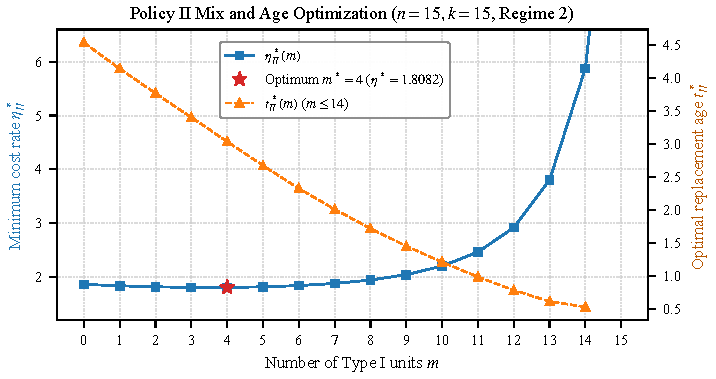
\includegraphics[width=0.78\textwidth]{../figures/figS3_policy2_minlp.pdf}
\caption{Synthetic Policy~II joint component-mix and replacement age optimization ($n = 15, k = 15$, Regime~2), yielding minimum $1.80818$ at $m^* = 4$ (near-tie $m = 3$ at $1.80835$).}
\label{fig:S3}
\end{figure}

\begin{figure}[htbp]
\centering
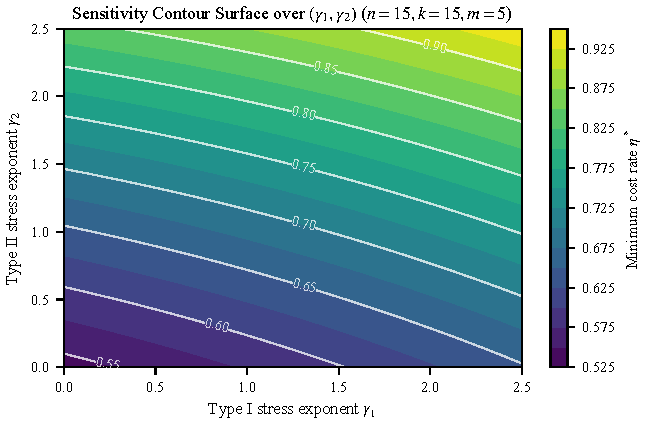
\includegraphics[width=0.72\textwidth]{../figures/figS4_contour_sensitivity.pdf}
\caption{Synthetic 2D contour sensitivity of minimum cost rate $\eta^*$ over $(\gamma_1, \gamma_2)$ ($n = 15, k = 15, m = 5$).}
\label{fig:S4}
\end{figure}

\clearpage
\section{Extended IEEE RTS-GMLC Grids (E1--E4)}
\label{sec:S3}

Tables~\ref{tab:S5}--\ref{tab:S8} archive extended results for the RTS-GMLC-parameterized peaking combustion-turbine (CT) and coal steam arrays \cite{barrows2020}, calibrated against GE Vernova GER-3620 Rev~P \cite{ger3620} and EIA AEO 2026 \cite{eia2026} (complete machine-readable CSV archives reside in \texttt{results/}). Specifically, Table~\ref{tab:S5} shows 13 extended E1/E2 mechanism rows from the 480-row \texttt{case\_E2\_mechanism\_branches.csv} archive ($\rho \in \{1.15, 1.10, 1.05, 1.03\}$) completely disjoint from Main Table~3 (spanning $k/W_0 \in \{0.60, 0.70, 0.80\}$ at $c_2/c_1 = 5$ across CT Areas~1--3 plus CT Areas~2--3 at $k/W_0 = 0.70, c_2/c_1 \in \{10, 20\}$); Table~\ref{tab:S6} reports all 80 E3 turning-point configurations; Table~\ref{tab:S7} details the E4 4D parameter-box summary across individual CT areas under the symmetric $\pm 1$ band ($3 \le m^* \le 5$); and Table~\ref{tab:S8} presents E2b asymmetric cross-branch sensitivity ($\gamma_1 \neq \gamma_2$) from the 720-row \texttt{case\_E2\_asymmetric\_gamma.csv} archive ($\rho \in \{1.15, 1.10, 1.03\}$) at $k/W_0 = 0.70, c_2/c_1 = 5, \rho = 1.15$.

\begin{table}[htbp]
\centering
\scriptsize
\setlength{\tabcolsep}{1.5pt}
\caption{Extended CT array Policy~I comparison completely disjoint from Main Table~3 ($c_2/c_1 = 5$ across $k/W_0 \in \{0.60, 0.70, 0.80\}$ for CT Areas~1--3, plus CT Areas~2--3 $c_2/c_1 \in \{10, 20\}$ at $k/W_0 = 0.70$), showing $t^*$ (h), $\eta^*$, CM savings gap $\mathrm{Gap} = [\eta(\infty)-\eta^*]/\eta(\infty)$, and naive $\gamma = 0$ penalty $\Delta\eta\%$.}
\label{tab:S5}
\begin{tabular*}{\textwidth}{@{\extracolsep{\fill}}lcc|cc|cccc|ccc|cc@{}}
\toprule
 & & & \multicolumn{2}{c|}{$\gamma = 0$ (E1)} & \multicolumn{4}{c|}{Rotor $\rho=1.15$ ($\gamma=4.96$)} & \multicolumn{3}{c|}{HGP $\rho=1.15$ ($\gamma=12.88$)} & \multicolumn{2}{c}{Rotor $\rho=1.03$ ($\gamma=23.45$)} \\
Array ($c_2/c_1$) & $k/W_0$ & $k$ & $t^*$ (h) & $\eta^*$ & $t^*$ (h) & $\eta^*$ & Gap & $\Delta\eta\%$ & $t^*$ (h) & $\eta^*$ & $\Delta\eta\%$ & $t^*$ (h) & $\Delta\eta\%$ \\
\midrule
CT Area 1 (5) & 0.60 & 279 & 230.64 & 0.006520 & 93.81 & 0.017109 & 32.19\% & 29.32\% & 63.38 & 0.041193 & 9.85\% & 93.51 & 0.86\% \\
CT Area 1 (5) & 0.70 & 326 & 164.17 & 0.010453 & 88.58 & 0.020203 & 26.10\% & 12.23\% & 64.46 & 0.041601 & 6.83\% & 93.58 & 0.56\% \\
CT Area 1 (5) & 0.80 & 372 & 115.89 & 0.019823 & 81.85 & 0.028323 & 15.58\% & 2.58\%  & 71.95 & 0.044547 & 1.94\% & 96.20 & 0.09\% \\
\midrule
CT Area 2 (5) & 0.60 & 345 & 243.05 & 0.006145 & 94.36 & 0.016025 & 36.85\% & 40.01\% & 52.29 & 0.040632 & 16.68\% & 75.80 & 2.03\% \\
CT Area 2 (5) & 0.70 & 403 & 173.15 & 0.009554 & 88.26 & 0.018803 & 31.56\% & 18.96\% & 52.73 & 0.041053 & 13.42\% & 75.83 & 1.60\% \\
CT Area 2 (5) & 0.80 & 460 & 119.25 & 0.016585 & 79.29 & 0.025185 & 21.81\% & 4.74\%  & 55.48 & 0.043375 & 6.61\%  & 76.66 & 0.71\% \\
\midrule
CT Area 3 (5) & 0.60 & 411 & 236.12 & 0.005919 & 93.29 & 0.015390 & 40.52\% & 47.33\% & 47.55 & 0.039739 & 23.71\% & 60.13 & 3.44\% \\
CT Area 3 (5) & 0.70 & 480 & 179.46 & 0.008476 & 87.22 & 0.017500 & 36.84\% & 28.00\% & 47.67 & 0.040120 & 20.79\% & 60.16 & 3.04\% \\
CT Area 3 (5) & 0.80 & 548 & 113.58 & 0.015325 & 73.74 & 0.023870 & 27.91\% & 7.53\%  & 48.46 & 0.042779 & 11.09\% & 60.93 & 1.60\% \\
\midrule
CT Area 2 (10) & 0.70 & 403 & 120.67 & 0.012735 & 61.55 & 0.025122 & 54.28\% & 31.55\% & 30.18 & 0.059654 & 43.54\% & 28.12 & 12.89\% \\
CT Area 2 (20) & 0.70 & 403 & 90.70  & 0.016281 & 46.15 & 0.032224 & 70.68\% & 43.14\% & 20.41 & 0.080964 & 87.79\% & 12.93 & 37.65\% \\
CT Area 3 (10) & 0.70 & 480 & 133.27 & 0.010933 & 64.21 & 0.022550 & 59.31\% & 48.70\% & 29.56 & 0.056033 & 61.92\% & 21.69 & 21.75\% \\
CT Area 3 (20) & 0.70 & 480 & 104.08 & 0.013676 & 50.17 & 0.028088 & 74.66\% & 67.47\% & 20.97 & 0.073607 & 123.77\% & 12.11 & 59.36\% \\
\bottomrule
\end{tabular*}
\end{table}

\begin{table}[htbp]
\centering
\scriptsize
\caption{Complete 80-configuration turning-point exponent $\gamma_{\mathrm{tp}}$ and $<1\%$ corrective-only threshold $\gamma_{\mathrm{CM},1\%}$ (E3; ``---'' denotes arrays already within $<1\%$ of corrective-only cost at $\gamma = 0$).}
\label{tab:S6}
\begin{tabular*}{\textwidth}{@{\extracolsep{\fill}}lcc|cc|cc|cc|cc@{}}
\toprule
 & & & \multicolumn{2}{c|}{$c_2/c_1 = 3$} & \multicolumn{2}{c|}{$c_2/c_1 = 5$} & \multicolumn{2}{c|}{$c_2/c_1 = 10$} & \multicolumn{2}{c}{$c_2/c_1 = 20$} \\
Array & $k/W_0$ & $k$ & $\gamma_{\mathrm{tp}}$ & $\gamma_{\mathrm{CM},1\%}$ & $\gamma_{\mathrm{tp}}$ & $\gamma_{\mathrm{CM},1\%}$ & $\gamma_{\mathrm{tp}}$ & $\gamma_{\mathrm{CM},1\%}$ & $\gamma_{\mathrm{tp}}$ & $\gamma_{\mathrm{CM},1\%}$ \\
\midrule
CT Area 1 & 0.50 & 233 & 7.69 & 13.98 & 10.82 & 25.42 & 15.23 & 42.43 & 19.67 & 59.71 \\
CT Area 1 & 0.60 & 279 & 7.69 & 12.84 & 10.82 & 25.42 & 15.23 & 42.43 & 19.67 & 59.71 \\
CT Area 1 & 0.70 & 326 & 7.69 & 12.84 & 11.78 & 25.42 & 15.23 & 42.43 & 19.67 & 59.71 \\
CT Area 1 & 0.80 & 372 & 6.48 & 10.82 & 9.93 & 23.34 & 15.23 & 42.43 & 19.67 & 59.71 \\
CT Area 1 & 0.90 & 419 & --- & 0.00 & --- & 0.00 & 30.15 & 38.96 & 46.21 & 59.71 \\
\midrule
CT Area 2 & 0.50 & 288 & 9.93 & 15.23 & 13.98 & 27.68 & 19.67 & 46.21 & 23.34 & 65.03 \\
CT Area 2 & 0.60 & 345 & 9.93 & 15.23 & 13.98 & 27.68 & 19.67 & 46.21 & 23.34 & 65.03 \\
CT Area 2 & 0.70 & 403 & 9.93 & 15.23 & 13.98 & 27.68 & 19.67 & 46.21 & 23.34 & 65.03 \\
CT Area 2 & 0.80 & 460 & 9.12 & 13.98 & 13.98 & 27.68 & 19.67 & 46.21 & 23.34 & 65.03 \\
CT Area 2 & 0.90 & 518 & --- & 0.00 & 9.12 & 23.34 & 15.23 & 46.21 & 21.43 & 65.03 \\
\midrule
CT Area 3 & 0.50 & 343 & 10.82 & 16.58 & 16.58 & 30.15 & 23.34 & 50.33 & 30.15 & 77.14 \\
CT Area 3 & 0.60 & 411 & 10.82 & 16.58 & 16.58 & 30.15 & 23.34 & 50.33 & 30.15 & 77.14 \\
CT Area 3 & 0.70 & 480 & 10.82 & 16.58 & 16.58 & 30.15 & 23.34 & 50.33 & 30.15 & 77.14 \\
CT Area 3 & 0.80 & 548 & 10.82 & 16.58 & 16.58 & 30.15 & 23.34 & 50.33 & 30.15 & 77.14 \\
CT Area 3 & 0.90 & 617 & --- & 0.00 & 9.93 & 25.42 & 18.06 & 50.33 & 25.42 & 77.14 \\
\midrule
Coal Area 1 & 0.50 & 385 & 4.23 & 5.95 & 6.48 & 9.93 & 9.12 & 15.23 & 11.78 & 21.43 \\
Coal Area 1 & 0.60 & 462 & 4.23 & 5.46 & 6.48 & 9.93 & 9.12 & 15.23 & 11.78 & 21.43 \\
Coal Area 1 & 0.70 & 539 & --- & 0.00 & 5.46 & 9.12 & 8.37 & 15.23 & 11.78 & 21.43 \\
Coal Area 1 & 0.80 & 616 & --- & 0.00 & --- & 0.00 & --- & 0.00 & --- & 0.00 \\
Coal Area 1 & 0.90 & 693 & --- & 0.00 & --- & 0.00 & --- & 0.00 & 15.23 & 19.67 \\
\bottomrule
\end{tabular*}
\end{table}

\begin{table}[htbp]
\centering
\scriptsize
\setlength{\tabcolsep}{1.2pt}
\caption{Complete 4D parameter-box consistency and interior regret summary by CT area and cost subset (E4, matching \texttt{case\_E4\_consistency\_summary.csv}; $m=4$ and $m=0$ regrets reported across interior cells $m^* \ge 1$).}
\label{tab:S7}
\begin{tabular*}{\textwidth}{@{\extracolsep{\fill}}llcccc|cc|cc@{}}
\toprule
 & & & & & & \multicolumn{2}{c|}{$m=4$ Regret} & \multicolumn{2}{c}{$m=0$ Regret} \\
Array & Subset & Pts & $m^*=0$ & $3\le m^*\le 5$ & $m^*\ge 1$ & Med. & Max & Med. & Max \\
\midrule
CT Area 1 & Full 4D Box      & 1250 & 78.08\% (976) & 10.80\% (135) & 21.92\% (274) & 1.29\% & 26.22\% & 3.38\% & 22.88\% \\
CT Area 1 & Symmetric ($r_{\mathrm{OM}}=1.00$) & 250  & 100.00\% (250) & 0.00\% (0) & 0.00\% (0) & --- & --- & --- & --- \\
CT Area 1 & EIA Slice ($r_{\mathrm{OM}}=1.96$) & 250  & 82.80\% (207) & 10.00\% (25) & 17.20\% (43) & 0.79\% & 18.98\% & 1.42\% & 7.54\% \\
CT Area 1 & Asymmetric ($r_{\mathrm{OM}}>1$)    & 1000 & 72.60\% (726) & 13.50\% (135) & 27.40\% (274) & 1.29\% & 26.22\% & 3.38\% & 22.88\% \\
\midrule
CT Area 2 & Full 4D Box      & 1250 & 77.20\% (965) & 8.88\% (111) & 22.80\% (285) & 1.95\% & 25.41\% & 4.00\% & 24.47\% \\
CT Area 2 & Symmetric ($r_{\mathrm{OM}}=1.00$) & 250  & 100.00\% (250) & 0.00\% (0) & 0.00\% (0) & --- & --- & --- & --- \\
CT Area 2 & EIA Slice ($r_{\mathrm{OM}}=1.96$) & 250  & 84.00\% (210) & 7.20\% (18) & 16.00\% (40) & 1.22\% & 13.43\% & 2.08\% & 6.27\% \\
CT Area 2 & Asymmetric ($r_{\mathrm{OM}}>1$)    & 1000 & 71.50\% (715) & 11.10\% (111) & 28.50\% (285) & 1.95\% & 25.41\% & 4.00\% & 24.47\% \\
\midrule
CT Area 3 & Full 4D Box      & 1250 & 72.32\% (904) & 8.72\% (109) & 27.68\% (346) & 1.76\% & 27.73\% & 4.39\% & 31.18\% \\
CT Area 3 & Symmetric ($r_{\mathrm{OM}}=1.00$) & 250  & 100.00\% (250) & 0.00\% (0) & 0.00\% (0) & --- & --- & --- & --- \\
CT Area 3 & EIA Slice ($r_{\mathrm{OM}}=1.96$) & 250  & 76.80\% (192) & 6.00\% (15) & 23.20\% (58) & 1.33\% & 7.65\% & 3.10\% & 12.17\% \\
CT Area 3 & Asymmetric ($r_{\mathrm{OM}}>1$)    & 1000 & 65.40\% (654) & 10.90\% (109) & 34.60\% (346) & 1.76\% & 27.73\% & 4.39\% & 31.18\% \\
\midrule
Pooled & Full 4D Box           & 3750 & 75.87\% (2845) & 9.47\% (355) & 24.13\% (905) & 1.61\% & 27.73\% & 3.90\% & 31.18\% \\
Pooled & EIA Slice ($r_{\mathrm{OM}}=1.96$) & 750  & 81.20\% (609) & 7.73\% (58) & 18.80\% (141) & 1.16\% & 18.98\% & 1.93\% & 12.17\% \\
Pooled & Policy I (No O\&M diff.) & 600 & 100.00\% (600) & 0.00\% (0) & 0.00\% (0) & --- & --- & --- & --- \\
\bottomrule
\end{tabular*}
\end{table}

\begin{table}[htbp]
\centering
\scriptsize
\caption{Asymmetric cross-branch sensitivity ($\gamma_1 \neq \gamma_2$) across Rotor ($\gamma=4.96$) and HGP ($\gamma=12.88$) CT branches at $k/W_0 = 0.70, c_2/c_1 = 5, \rho = 1.15$ (E2b, \texttt{case\_E2\_asymmetric\_gamma.csv}).}
\label{tab:S8}
\begin{tabular*}{\textwidth}{@{\extracolsep{\fill}}llcccccc@{}}
\toprule
Array & Branch Pair (T-I / T-II) & $\gamma_1, \gamma_2$ & $\mathrm{MTTF}$ (h) & $t^*$ (h) & $\eta^*$ & CM Gap (\%) & Naive $\Delta\eta\%$ \\
\midrule
CT Area 1 & Rotor / Rotor & 4.96, 4.96   & 182.89 & 88.58 & 0.020203 & 26.10\% & 12.23\% \\
CT Area 1 & HGP / Rotor   & 12.88, 4.96  & 155.43 & 80.75 & 0.026264 & 18.36\% & 9.51\%  \\
CT Area 1 & Rotor / HGP   & 4.96, 12.88  & 117.49 & 63.62 & 0.036917 & 13.25\% & 9.49\%  \\
CT Area 1 & HGP / HGP     & 12.88, 12.88 & 108.25 & 64.46 & 0.041601 & 9.94\%  & 6.83\%  \\
\midrule
CT Area 2 & Rotor / Rotor & 4.96, 4.96   & 181.99 & 88.26 & 0.018803 & 31.56\% & 18.96\% \\
CT Area 2 & HGP / Rotor   & 12.88, 4.96  & 148.14 & 70.79 & 0.025668 & 23.95\% & 18.30\% \\
CT Area 2 & Rotor / HGP   & 4.96, 12.88  & 111.17 & 55.26 & 0.037087 & 17.54\% & 16.04\% \\
CT Area 2 & HGP / HGP     & 12.88, 12.88 & 103.76 & 52.73 & 0.041053 & 14.81\% & 13.42\% \\
\midrule
CT Area 3 & Rotor / Rotor & 4.96, 4.96   & 180.44 & 87.22 & 0.017500 & 36.84\% & 28.00\% \\
CT Area 3 & HGP / Rotor   & 12.88, 4.96  & 154.83 & 74.04 & 0.022518 & 30.27\% & 25.95\% \\
CT Area 3 & Rotor / HGP   & 4.96, 12.88  & 106.42 & 50.68 & 0.036774 & 21.73\% & 23.03\% \\
CT Area 3 & HGP / HGP     & 12.88, 12.88 & 100.13 & 47.67 & 0.040120 & 19.65\% & 20.79\% \\
\bottomrule
\end{tabular*}
\end{table}

\section{Extended Non-Zero Replacement Duration Grid (E6)}
\label{sec:S4}

Table~\ref{tab:S9} compiles 51 representative E6 downtime evaluations under unpenalized downtime ($c_d = 0$) at $k/W_0 = 0.70, c_2/c_1 = 5$ across CT Areas~1--3 (using lower bound \texttt{U55} $31\;\text{h}$, unit-count-weighted array mean \texttt{WeightedAvg}, e.g., $37.91\;\text{h}$ for CT Area~1, and upper bound \texttt{U20} $50\;\text{h}$ as $d_{CM}$) and Coal Area~1 ($40\;\text{h}$) for continuous duty ($\delta = 1.00$, 39 rows) and peaking duty ($\delta = 0.10$, 12 CT rows including the \texttt{U55} lower-bound rows at $-0.39\%$ and $-9.78\%$) across $\gamma \in \{0.00, 4.96, 12.88, 23.45, 60.90\}$. Across the full 3,360-row E6 archive (\texttt{case\_E6\_downtime\_sensitivity.csv}, $c_d = 0$), nonzero durations dilute cycle denominators and reduce calendar cost rates in all $2{,}628$ finite cases ($4.31\%$--$94.11\%$ at $\delta = 1.00$; $0.45\%$--$46.02\%$ at $\delta = 0.10$). Denominator inversion $c_1/d_{PM} < c_2/(\delta^{-1}\mathrm{MTTF} + d_{CM})$ affects $815$ of $2{,}628$ finite rows: $775$ continuous rows ($\delta = 1.00$) and $40$ peaking rows ($\delta = 0.10$) at $c_2/c_1 = 20$ spanning $\gamma \in \{7.27, 12.88, 18.89, 23.45, 60.90\}$ (up to $-96.76\%$). Conversely, pricing downtime at $c_d = \delta c_2 / \mathrm{MTTF}$ yields $0/2{,}628$ inversions and modestly lengthens CT $t^*$ at $k/W_0 = 0.70, c_2/c_1 = 5$ by $+0.92\%$--$+17.46\%$ ($\delta = 1.00$) and $+0.12\%$--$+3.12\%$ ($\delta = 0.10$; verified in \texttt{supplemental\_sensitivity\_checks.csv}).

\begin{table}[htbp]
\centering
\scriptsize
\setlength{\tabcolsep}{1.8pt}
\caption{Representative E6 replacement and repair duration sensitivity ($c_d = 0$) at $k/W_0 = 0.70, c_2/c_1 = 5$ across reported RTS-GMLC MTTR bases and duty factors ($\delta \in \{1.00, 0.10\}$).}
\label{tab:S9}
\begin{tabular*}{\textwidth}{@{\extracolsep{\fill}}llcc|cc|ccc|ccc@{}}
\toprule
 & & & & \multicolumn{2}{c|}{Instantaneous ($0,0$)} & \multicolumn{3}{c|}{$d_{PM} = d_{CM}/2$} & \multicolumn{3}{c}{$d_{PM} = d_{CM}$} \\
Array & $d_{CM}$ Basis & $\delta$ & $\gamma$ & $t^*$ & $\eta_{\mathrm{cal}}^*$ & $t^*$ & $\Delta t^*$ & $\eta_{\mathrm{cal}}^*$ & $t^*$ & $\Delta t^*$ & $\eta_{\mathrm{cal}}^*$ \\
\midrule
CT Area 1 & U55 (31 h)    & 1.00 & 0.00  & 164.17 & 0.010453 & 154.49 & $-5.90\%$  & 0.009360 & 140.78 & $-14.25\%$ & 0.008628 \\
CT Area 1 & WeightedAvg   & 1.00 & 0.00  & 164.17 & 0.010453 & 152.49 & $-7.12\%$  & 0.009143 & 136.52 & $-16.84\%$ & 0.008282 \\
CT Area 1 & U20 (50 h)    & 1.00 & 0.00  & 164.17 & 0.010453 & 149.12 & $-9.17\%$  & 0.008783 & 129.72 & $-20.99\%$ & 0.007725 \\
CT Area 1 & U55 (31 h)    & 1.00 & 4.96  & 88.58  & 0.020203 & 78.10  & $-11.84\%$ & 0.016500 & 65.40  & $-26.17\%$ & 0.014227 \\
CT Area 1 & WeightedAvg   & 1.00 & 4.96  & 88.58  & 0.020203 & 76.10  & $-14.10\%$ & 0.015828 & 61.92  & $-30.10\%$ & 0.013246 \\
CT Area 1 & U20 (50 h)    & 1.00 & 4.96  & 88.58  & 0.020203 & 72.84  & $-17.77\%$ & 0.014757 & 56.76  & $-35.92\%$ & 0.011766 \\
CT Area 1 & U55 (31 h)    & 1.00 & 12.88 & 64.46  & 0.041601 & 40.44  & $-37.27\%$ & 0.029484 & 24.28  & $-62.33\%$ & 0.022793 \\
CT Area 1 & WeightedAvg   & 1.00 & 12.88 & 64.46  & 0.041601 & 37.13  & $-42.40\%$ & 0.027481 & 21.34  & $-66.89\%$ & 0.020182 \\
CT Area 1 & U20 (50 h)    & 1.00 & 12.88 & 64.46  & 0.041601 & 32.45  & $-49.65\%$ & 0.024437 & 17.75  & $-72.47\%$ & 0.016660 \\
CT Area 1 & U55 (31 h)    & 1.00 & 23.45 & 93.58  & 0.060382 & 36.27  & $-61.24\%$ & 0.040463 & 8.14   & $-91.30\%$ & 0.029004 \\
CT Area 1 & WeightedAvg   & 1.00 & 23.45 & 93.58  & 0.060382 & 29.80  & $-68.15\%$ & 0.037187 & 6.06   & $-93.52\%$ & 0.024538 \\
CT Area 1 & U20 (50 h)    & 1.00 & 23.45 & 93.58  & 0.060382 & 20.54  & $-78.05\%$ & 0.032166 & 4.34   & $-95.37\%$ & 0.019156 \\
CT Area 1 & U55 (31 h)    & 1.00 & 60.90 & $\infty$ & 0.077036 & $\infty$ & ---      & 0.052135 & 0.66   & ---        & 0.032191 \\
CT Area 1 & U20 (50 h)    & 1.00 & 60.90 & $\infty$ & 0.077036 & 5.15   & ---        & 0.038498 & 0.50   & ---        & 0.020081 \\
\midrule
CT Area 2 & U55 (31 h)    & 1.00 & 0.00  & 173.15 & 0.009554 & 164.19 & $-5.17\%$  & 0.008618 & 151.34 & $-12.59\%$ & 0.007976 \\
CT Area 2 & U20 (50 h)    & 1.00 & 0.00  & 173.15 & 0.009554 & 159.19 & $-8.06\%$  & 0.008119 & 140.80 & $-18.68\%$ & 0.007188 \\
CT Area 2 & U55 (31 h)    & 1.00 & 4.96  & 88.26  & 0.018803 & 79.80  & $-9.59\%$  & 0.015458 & 69.10  & $-21.71\%$ & 0.013366 \\
CT Area 2 & U20 (50 h)    & 1.00 & 4.96  & 88.26  & 0.018803 & 75.44  & $-14.53\%$ & 0.013880 & 61.47  & $-30.35\%$ & 0.011141 \\
CT Area 2 & U55 (31 h)    & 1.00 & 12.88 & 52.73  & 0.041053 & 37.29  & $-29.27\%$ & 0.028560 & 25.18  & $-52.24\%$ & 0.021927 \\
CT Area 2 & U20 (50 h)    & 1.00 & 12.88 & 52.73  & 0.041053 & 31.59  & $-40.09\%$ & 0.023619 & 19.58  & $-62.87\%$ & 0.016146 \\
CT Area 2 & U55 (31 h)    & 1.00 & 23.45 & 75.83  & 0.063888 & 27.04  & $-64.34\%$ & 0.041195 & 8.70   & $-88.53\%$ & 0.028308 \\
CT Area 2 & U20 (50 h)    & 1.00 & 23.45 & 75.83  & 0.063888 & 15.21  & $-79.94\%$ & 0.031892 & 5.53   & $-92.71\%$ & 0.018869 \\
CT Area 2 & U55 (31 h)    & 1.00 & 60.90 & $\infty$ & 0.084992 & 19.07 & ---       & 0.054507 & 0.50   & ---        & 0.032190 \\
CT Area 2 & U20 (50 h)    & 1.00 & 60.90 & $\infty$ & 0.084992 & 4.51  & ---        & 0.038908 & 0.50   & ---        & 0.020079 \\
\midrule
CT Area 3 & U55 (31 h)    & 1.00 & 0.00  & 179.46 & 0.008476 & 172.81 & $-3.71\%$  & 0.007701 & 162.98 & $-9.18\%$  & 0.007148 \\
CT Area 3 & U20 (50 h)    & 1.00 & 0.00  & 179.46 & 0.008476 & 169.02 & $-5.82\%$  & 0.007285 & 154.64 & $-13.83\%$ & 0.006488 \\
CT Area 3 & U55 (31 h)    & 1.00 & 4.96  & 87.22  & 0.017500 & 80.58  & $-7.61\%$  & 0.014462 & 72.02  & $-17.43\%$ & 0.012515 \\
CT Area 3 & U20 (50 h)    & 1.00 & 4.96  & 87.22  & 0.017500 & 77.12  & $-11.58\%$ & 0.013027 & 65.73  & $-24.64\%$ & 0.010499 \\
CT Area 3 & U55 (31 h)    & 1.00 & 12.88 & 47.67  & 0.040120 & 35.94  & $-24.60\%$ & 0.027692 & 26.05  & $-45.36\%$ & 0.021193 \\
CT Area 3 & U20 (50 h)    & 1.00 & 12.88 & 47.67  & 0.040120 & 31.37  & $-34.19\%$ & 0.022902 & 21.15  & $-55.63\%$ & 0.015703 \\
CT Area 3 & U55 (31 h)    & 1.00 & 23.45 & 60.16  & 0.066851 & 21.21  & $-64.75\%$ & 0.040958 & 9.44   & $-84.31\%$ & 0.027735 \\
CT Area 3 & U20 (50 h)    & 1.00 & 23.45 & 60.16  & 0.066851 & 14.36  & $-76.14\%$ & 0.031321 & 6.43   & $-89.31\%$ & 0.018624 \\
CT Area 3 & U55 (31 h)    & 1.00 & 60.90 & $\infty$ & 0.092762 & 14.96 & ---       & 0.056028 & 0.50   & ---        & 0.032083 \\
CT Area 3 & U20 (50 h)    & 1.00 & 60.90 & $\infty$ & 0.092762 & 2.74  & ---        & 0.039250 & 0.50   & ---        & 0.020012 \\
\midrule
CT Area 1 & U20 (50 h)    & 0.10 & 0.00  & 164.17 & 0.001045 & 162.53 & $-1.00\%$  & 0.001026 & 159.86 & $-2.63\%$  & 0.001013 \\
CT Area 1 & U20 (50 h)    & 0.10 & 4.96  & 88.58  & 0.002020 & 86.70  & $-2.12\%$  & 0.001952 & 83.74  & $-5.46\%$  & 0.001904 \\
CT Area 1 & U20 (50 h)    & 0.10 & 12.88 & 64.46  & 0.004160 & 59.27  & $-8.04\%$  & 0.003923 & 51.89  & $-19.50\%$ & 0.003793 \\
CT Area 1 & U20 (50 h)    & 0.10 & 23.45 & 93.58  & 0.006038 & 77.65  & $-17.02\%$ & 0.005643 & 59.65  & $-36.26\%$ & 0.005522 \\
CT Area 1 & U20 (50 h)    & 0.10 & 60.90 & $\infty$ & 0.007704 & $\infty$ & ---      & 0.007153 & $\infty$ & ---      & 0.007153 \\
CT Area 3 & U20 (50 h)    & 0.10 & 0.00  & 179.46 & 0.000848 & 178.34 & $-0.62\%$  & 0.000834 & 176.52 & $-1.64\%$  & 0.000824 \\
CT Area 3 & U20 (50 h)    & 0.10 & 4.96  & 87.22  & 0.001750 & 86.06  & $-1.34\%$  & 0.001694 & 84.20  & $-3.47\%$  & 0.001651 \\
CT Area 3 & U20 (50 h)    & 0.10 & 12.88 & 47.67  & 0.004012 & 45.28  & $-5.02\%$  & 0.003757 & 41.78  & $-12.36\%$ & 0.003588 \\
CT Area 3 & U20 (50 h)    & 0.10 & 23.45 & 60.16  & 0.006685 & 50.03  & $-16.84\%$ & 0.006161 & 36.75  & $-38.91\%$ & 0.005924 \\
CT Area 3 & U20 (50 h)    & 0.10 & 60.90 & $\infty$ & 0.009276 & $\infty$ & ---      & 0.008489 & $\infty$ & ---      & 0.008489 \\
CT Area 3 & U55 (31 h)    & 0.10 & 0.00  & 179.46 & 0.000848 & 178.77 & $-0.39\%$  & 0.000839 & 177.62 & $-1.02\%$  & 0.000833 \\
CT Area 2 & U55 (31 h)    & 0.10 & 23.45 & 75.83  & 0.006389 & 68.42  & $-9.78\%$  & 0.006101 & 57.93  & $-23.60\%$ & 0.006011 \\
\midrule
Coal Area 1 & U76/155 (40 h) & 1.00 & 0.00  & 307.29 & 0.009857 & 267.10 & $-13.08\%$ & 0.008876 & 214.18 & $-30.30\%$ & 0.008370 \\
Coal Area 1 & U76/155 (40 h) & 1.00 & 4.96  & 212.68 & 0.015397 & 166.88 & $-21.54\%$ & 0.013149 & 116.22 & $-45.36\%$ & 0.011952 \\
Coal Area 1 & U76/155 (40 h) & 1.00 & 12.88 & $\infty$ & 0.022143 & $\infty$ & ---    & 0.018811 & 71.06  & ---        & 0.017355 \\
Coal Area 1 & U76/155 (40 h) & 1.00 & 23.45 & $\infty$ & 0.024764 & $\infty$ & ---    & 0.020669 & $\infty$ & ---      & 0.020669 \\
Coal Area 1 & U76/155 (40 h) & 1.00 & 60.90 & $\infty$ & 0.025809 & $\infty$ & ---    & 0.021392 & $\infty$ & ---      & 0.021392 \\
\bottomrule
\end{tabular*}
\end{table}

\begin{thebibliography}{9}
\bibitem{wu1994} Wu JS, Chen RJ. An algorithm for computing the reliability of weighted-k-out-of-n systems. IEEE Transactions on Reliability 1994; 43 (2): 327-328. doi: 10.1109/24.295016
\bibitem{nakagawa2005} Nakagawa T. Maintenance Theory of Reliability. London, UK: Springer-Verlag, 2005. doi: 10.1007/1-84628-221-7
\bibitem{eryilmaz2014two} Eryilmaz S, Sarikaya K. Modeling and analysis of weighted-k-out-of-n:G system consisting of two different types of components. Proceedings of the Institution of Mechanical Engineers, Part O: Journal of Risk and Reliability 2014; 228 (3): 265-271. doi: 10.1177/1748006X13515647
\bibitem{eryilmaz2018} Eryilmaz S. The number of failed components in a k-out-of-n system consisting of multiple types of components. Reliability Engineering \& System Safety 2018; 175: 246-250. doi: 10.1016/j.ress.2018.03.027
\bibitem{barrows2020} Barrows C, Preston E, Staid A, Stephen G, Watson JP et al. The IEEE Reliability Test System: a proposed 2019 update. IEEE Transactions on Power Systems 2020; 35 (1): 119-127. doi: 10.1109/tpwrs.2019.2925557
\bibitem{ger3620} Beagle D, Moran B, McDufford M, Merine M. Heavy-duty gas turbine operating and maintenance considerations. Technical Report GER-3620 Rev P. Atlanta, GA, USA: GE Vernova, 2021.
\bibitem{eia2026} U.S. Energy Information Administration. Assumptions to the Annual Energy Outlook 2026: Electricity Market Module. Washington, DC, USA: U.S. Department of Energy, 2026.
\end{thebibliography}

\end{document}
